%% using aastex version 6.3
\documentclass[twocolumn]{aastex63}

\newcommand{\vdag}{(v)^\dagger}
\newcommand\aastex{AAS\TeX}
\newcommand\latex{La\TeX}

%%%%%%%%%%%%%%%%%%%%%%%%%%%%%%%%%%%%%%%%%%%%%%%%%%%%%%%%%%%%%%%%%%%%%%%%%%%%%%%%
%%
%% The following section defines new commands for comments from co-authors
%%
\definecolor{DarkOrange}{RGB}{204, 85, 0}
\definecolor{LincolnGreen}{RGB}{17, 102, 0}
\def\ion#1#2{#1$\;${\footnotesize\rm{#2}}\relax}

\newcommand{\kate}[1]{{\color{red} KM: {#1}}}
\newcommand{\steve}[1]{{\color{purple} SS: {#1}}}

\newcommand{\abi}[1]{{\color{LincolnGreen} AP: {#1}}}
\newcommand{\yy}[1]{{\color{blue} YY: {#1}}}
\newcommand{\aam}[1]{{\color{DarkOrange} aam: {#1}}}
\newcommand{\stockholm}[1]{{\color{cyan} stockholm: {#1}}}
\newcommand{\todo}[1]{{\color{magenta} to-do: {#1}}}

\newcommand{\rztf}{$r_\mathrm{ZTF}$}
\newcommand{\gztf}{$g_\mathrm{ZTF}$}
\newcommand{\iztf}{$i_\mathrm{ZTF}$}
\newcommand{\tfl}{$t_\mathrm{fl}$}
\newcommand{\trise}{$t_\mathrm{rise}$}
\newcommand{\tbmax}{$t_{B,\mathrm{max}}$}
\newcommand{\kms}{km\,s$^{-1}$}

\newcommand{\sn}{SN\,2019yvq}

%%
%%%%%%%%%%%%%%%%%%%%%%%%%%%%%%%%%%%%%%%%%%%%%%%%%%%%%%%%%%%%%%%%%%%%%%%%%%%%%%%%

%% Reintroduced the \received and \accepted commands from AASTeX v5.2
\received{\today}
\revised{}
\accepted{}
%% Command to document which AAS Journal the manuscript was submitted to.
%% Adds "Submitted to " the argument.
\submitjournal{ApJ}

%% For manuscript that include authors in collaborations, AASTeX v6.3
%% builds on the \collaboration command to allow greater freedom to 
%% keep the traditional author+affiliation information but only show
%% subsets. The \collaboration command now must appear AFTER the group
%% of authors in the collaboration and it takes TWO arguments. The last
%% is still the collaboration identifier. The text given in this
%% argument is what will be shown in the manuscript. The first argument
%% is the number of author above the \collaboration command to show with
%% the collaboration text. If there are authors that are not part of any
%% collaboration the \nocollaboration command is used. This command takes
%% one argument which is also the number of authors above to show. A
%% dashed line is shown to indicate no collaboration. This example manuscript
%% shows how these commands work to display specific set of authors 
%% on the front page.
%%
%% For manuscript without any need to use \collaboration the 
%% \AuthorCollaborationLimit command from v6.2 can still be used to 
%% show a subset of authors.
%
%\AuthorCollaborationLimit=2
%
%% will only show Schwarz & Muench on the front page of the manuscript
%% (assuming the \collaboration and \nocollaboration commands are
%% commented out).
%%
%% Note that all of the author will be shown in the published article.
%% This feature is meant to be used prior to acceptance to make the
%% front end of a long author article more manageable. Please do not use
%% this functionality for manuscripts with less than 20 authors. Conversely,
%% please do use this when the number of authors exceeds 40.
%%
%% Use \allauthors at the manuscript end to show the full author list.
%% This command should only be used with \AuthorCollaborationLimit is used.

%% The following command can be used to set the latex table counters.  It
%% is needed in this document because it uses a mix of latex tabular and
%% AASTeX deluxetables.  In general it should not be needed.
%\setcounter{table}{1}

%%%%%%%%%%%%%%%%%%%%%%%%%%%%%%%%%%%%%%%%%%%%%%%%%%%%%%%%%%%%%%%%%%%%%%%%%%%%%%%%
%%
%% The following section outlines numerous optional output that
%% can be displayed in the front matter or as running meta-data.
%%
%% If you wish, you may supply running head information, although
%% this information may be modified by the editorial offices.
\shorttitle{\sn\ is Fun and Cool}
\shortauthors{Miller et al.}
%%
%% You can add a light gray and diagonal water-mark to the first page 
%% with this command:
\watermark{DRAFT}
%% where "text", e.g. DRAFT, is the text to appear.  If the text is 
%% long you can control the water-mark size with:
%% \setwatermarkfontsize{dimension}
%% where dimension is any recognized LaTeX dimension, e.g. pt, in, etc.
%%
%%%%%%%%%%%%%%%%%%%%%%%%%%%%%%%%%%%%%%%%%%%%%%%%%%%%%%%%%%%%%%%%%%%%%%%%%%%%%%%%
\graphicspath{{./}{figures/}}
%% This is the end of the preamble.  Indicate the beginning of the
%% manuscript itself with \begin{document}.

\begin{document}

\title{\sn\  }

%% LaTeX will automatically break titles if they run longer than
%% one line. However, you may use \\ to force a line break if
%% you desire. In v6.3 you can include a footnote in the title.

%% A significant change from earlier AASTEX versions is in the structure for 
%% calling author and affiliations. The change was necessary to implement 
%% auto-indexing of affiliations which prior was a manual process that could 
%% easily be tedious in large author manuscripts.
%%
%% The \author command is the same as before except it now takes an optional
%% argument which is the 16 digit ORCID. The syntax is:
%% \author[xxxx-xxxx-xxxx-xxxx]{Author Name}
%%
%% This will hyperlink the author name to the author's ORCID page. Note that
%% during compilation, LaTeX will do some limited checking of the format of
%% the ID to make sure it is valid. If the "orcid-ID.png" image file is 
%% present or in the LaTeX pathway, the OrcID icon will appear next to
%% the authors name.
%%
%% Use \affiliation for affiliation information. The old \affil is now aliased
%% to \affiliation. AASTeX v6.3 will automatically index these in the header.
%% When a duplicate is found its index will be the same as its previous entry.
%%
%% Note that \altaffilmark and \altaffiltext have been removed and thus 
%% can not be used to document secondary affiliations. If they are used latex
%% will issue a specific error message and quit. Please use multiple 
%% \affiliation calls for to document more than one affiliation.
%%
%% The new \altaffiliation can be used to indicate some secondary information
%% such as fellowships. This command produces a non-numeric footnote that is
%% set away from the numeric \affiliation footnotes.  NOTE that if an
%% \altaffiliation command is used it must come BEFORE the \affiliation call,
%% right after the \author command, in order to place the footnotes in
%% the proper location.
%%
%% Use \email to set provide email addresses. Each \email will appear on its
%% own line so you can put multiple email address in one \email call. A new
%% \correspondingauthor command is available in V6.3 to identify the
%% corresponding author of the manuscript. It is the author's responsibility
%% to make sure this name is also in the author list.
%%
%% While authors can be grouped inside the same \author and \affiliation
%% commands it is better to have a single author for each. This allows for
%% one to exploit all the new benefits and should make book-keeping easier.
%%
%% If done correctly the peer review system will be able to
%% automatically put the author and affiliation information from the manuscript
%% and save the corresponding author the trouble of entering it by hand.

% \author[0000-0001-9515-478X]{A.~A.~Miller}
% \affiliation{Center for Interdisciplinary Exploration and Research in Astrophysics (CIERA) and Department of Physics and Astronomy, Northwestern University, 2145 Sheridan Road, Evanston, IL 60208, USA}
% \affiliation{The Adler Planetarium, Chicago, IL 60605, USA}
% \email{amiller@northwestern.edu}

\author{ZTF}

\author{et al.}

%% Note that the \and command from previous versions of AASTeX is now
%% depreciated in this version as it is no longer necessary. AASTeX 
%% automatically takes care of all commas and "and"s between authors names.

%% Mark off the abstract in the ``abstract'' environment. 
\begin{abstract}

\todo{Write the abstract}

\end{abstract}

%% Keywords should appear after the \end{abstract} command. 
%% See the online documentation for the full list of available subject
%% keywords and the rules for their use.
\keywords{}

\section{Introduction} \label{sec:intro}

\todo{write it; define and include references for ZTF}

\section{Discovery and Observations}\label{sec:obs}

\sn\ was discovered by K.~Itagaki, and detected at an unfiltered magnitude of
16.7\,mag, in an image obtained on 2019 Dec 28.74 UT\footnote{UT times are
used throughout this paper}. The transient candidate was announced
$\sim$2\,hr later on the Transient Name Server (TNS), and given the
designation AT\,2019yvq \citep{Itagaki19}. Susequent spectroscopic
observations confirmed the SN nature of the transient, with initial reports
that the event was a SN Ib/c \citep{Kawabata20}, but later reports classified
the event as a SN Ia \todo{create refs for Prentice obs}. These spectroscopic
observations also showed \sn\ to be at the same redshift as NGC\,4441, its
host galaxy.

\subsection{ZTF Photometric Observations}

ZTF simulataneously conducts multiple time-domain surveys using the ZTF
camera on the the Palomar Oschin Schmidt 48 inch (P48) telescope. \sn\ was
first detected by ZTF on 2019 Dec 29.46, as part of the ZTF public survey
(see \citealt{Bellm19a}). The automated ZTF pipeline \citep{Masci19}
automatically detected \sn, which passed internal thresholds (e.g.,
\citealt{Mahabal19}), leading to the production and disemination of a
real-time alert \citep{Patterson19}. The public alert included the position,
$\alpha = 12^{\mathrm{h}}27\arcmin21\farcs836$, $\delta =
+64\degr47\arcmin59\farcs87$ (J2000), and brightness, \rztf$ =
17.14\pm0.05$\,mag, which, together with the \citet{Itagaki19} discovery
report suggested the SN was fading. Continued monitoring with ZTF, and
follow-up with other telescopes, confirmed a spectacular decline in the early
emission from \sn\ (Figure~\ref{fig:p48}).

\begin{figure}
    \centering
    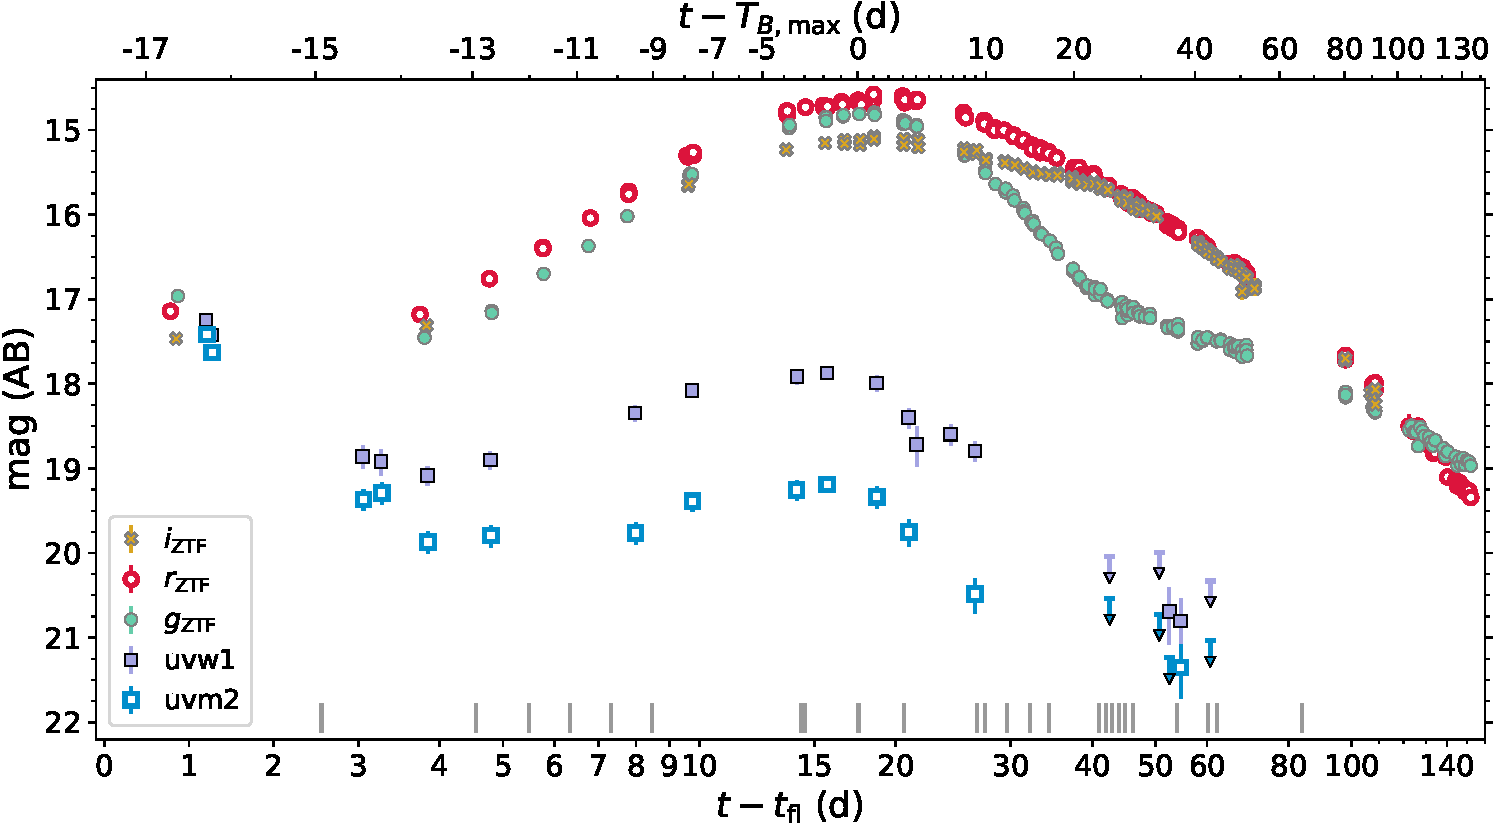
\includegraphics[width=3.5in]{./figures/P48_lc.pdf}
    %
    \caption{Photometric evolution of \sn, highlighting the initial decline
    observed in the light curve. \gztf, \rztf, and \iztf\ observations are
    shown as filled green circles, open red circles, and filled golden
    crosses, respectively. UVOT $u$ and $uvw2$ are The lower axis shows time
    measured in rest-frame days relative to \tfl, while the upper axis shows
    time relative to B-band maximum. Note that the horizontal axis is shown
    with a linear scale from $0\,\mathrm{d} \le t - t_\mathrm{fl} \le 3$\,d
    and a log scale for $t - t_\mathrm{fl} > 3$\,d. Vertical black ticks show
    epochs of spectroscopic observations. \todo{add marks for dates of
    spectra}}
    %
    \label{fig:p48}
\end{figure}

The field of \sn\ was additionally observed by ZTF with nearly a nightly
cadence as part of the ZTF partnership Uniform Depth Survey (ZUDS;
D.~Goldstein et al., in prep.). Using images obtained as part of the ZUDS
program, we perform forced PSF photometry at the location of \sn\ following
the procedure described in \citet{Yao19}.\footnote{Images obtained as part of
the ZTF public survey have not been released, preventing us from applying our
forced-PSF measurements. We therefore only include forced-PSF measurements in
the analysis described herein, though we note that our measurements are
largely consistent with those provided in the public alerts.} The evolution
of \sn\ in the \gztf, \rztf, and \iztf\ filters is shown in
Figure~\ref{fig:p48}.

\subsection{Other Photometric Observations}

Ultraviolet (UV) observations of \sn\ were obtained with the
Ultra-Violet/Optical Telescope (UVOT; \citet{Roming05}) onboard the Neil
Gehrels Swift Observatory (hereafter \textit{Swift}; \citealt{Gehrels04})
following a time-of-opportunity request by D.~Hiramatsu. For clarity, we only
show the \textit{Swift} $u$ and $uvw2$ light curves in Figure~\ref{fig:p48}.
\textit{Swift}/UVOT observations show that the initial decline seen in the
optical is even more dramatic in the UV.

We use a second-order polynomial to model the UVOT $b$-band light curve near
peak (including observations between JD$> 2,458,855.5$ and JD$<
2,458,871.5$). From the fit we estimate the time of $B$-band maximum \tbmax$
= 2,458,863.83 \pm 0.21$\,JD and that \sn\ peaked at $B = 14.98 \pm
0.03$\,mag (this estimate has not been corrected for extinction).

\subsection{Optical Spectroscopy}

Spectroscopic observations of \sn\ were taken with a variety of telescopes
and instruments over multiple epochs beginning $\sim$3\,d after discovery and
continuing through $\sim$3\,wk after \tbmax \todo{update these numbers}. An
observing log is listed in Table~\ref{tab:spectra}. The spectra were reduced
using standard procedures in \texttt{IDL}/\texttt{Python}/\texttt{Matlab}.
The optical spectral evolution of \sn\ is illustrated in
Figure~\ref{fig:spec_evo}.

\begin{figure}
    \centering
    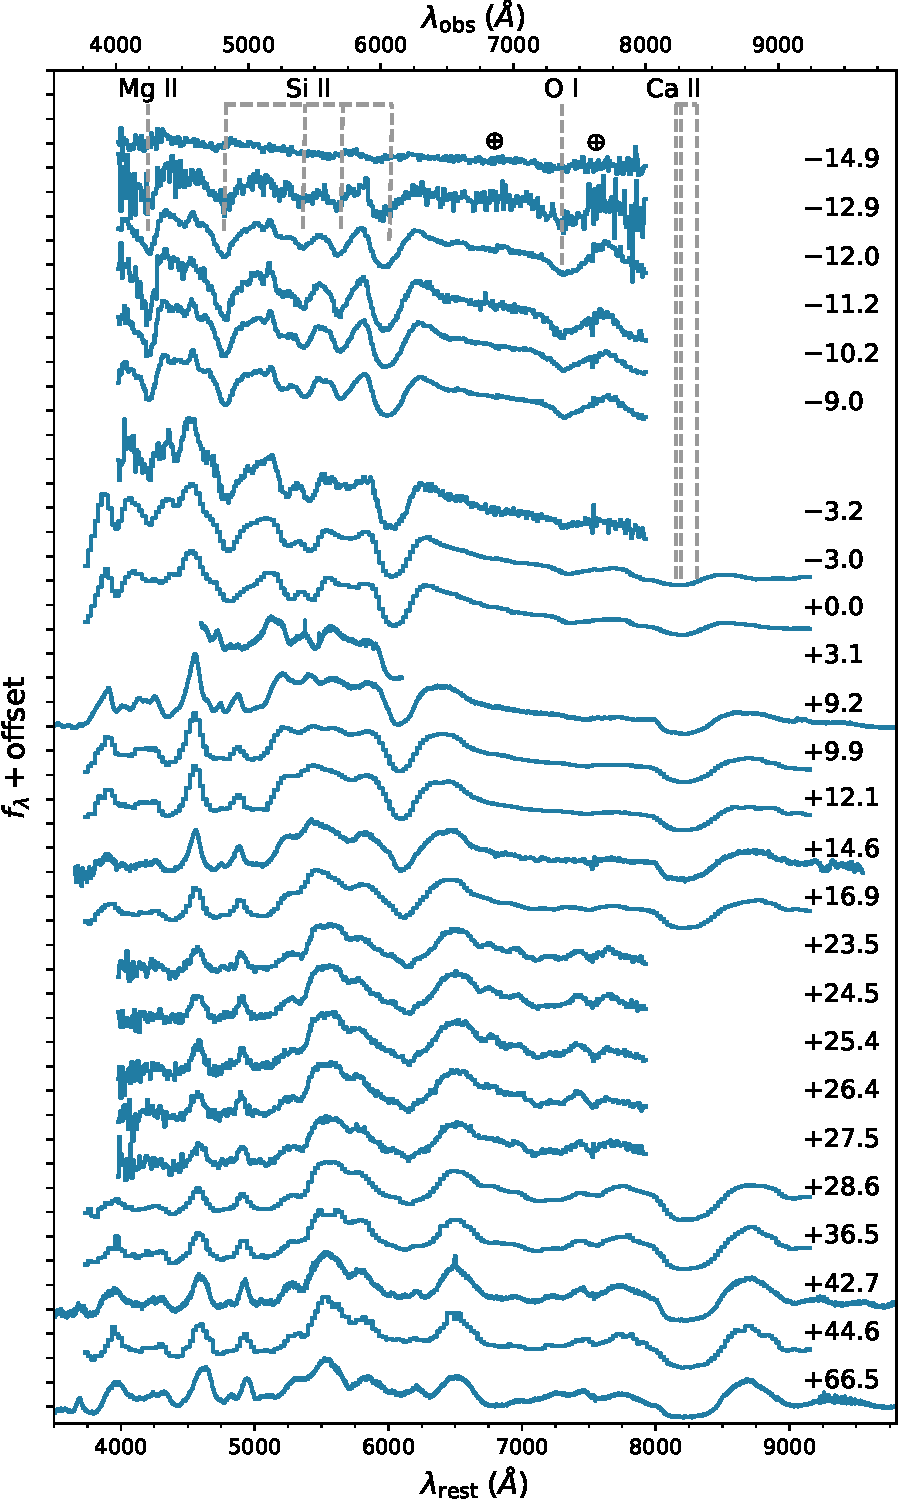
\includegraphics[width=3.5in]{./figures/spec_evo.pdf}
    %
    \caption{Observed spectral sequence of \sn. Spectra have been normalized
    by their median flux between 7200 \AA\ and 7400 \AA. The phase of each
    observation relative to \tbmax\ is shown to the right of the individual
    spectra. Prominent spectral features from intermediate mass elements are
    highlighted with vertical dashed lines. Some of the spectra feature
    imperfect Telluric subtractions, giving rise to the non-smooth features
    around $\lambda_\mathrm{obs} \approx 7600$\,\AA.}
    %
    \label{fig:spec_evo}
\end{figure}


\section{Analysis}\label{sec:analysis}

\subsection{NGC\,4441: the Host of \sn}

NGC\,4441 is the host galaxy of \sn. SDSS spectroscopic measurements of the
nucleus of NGC\,4441 yield a heliocentric-recession velocity of 2663\,\kms\
($z_\mathrm{helio} = 0.00888$; \citealt{Abolfathi18}) and a
\texttt{STARBURST} classification for NGC\,4441. Using the 2M++ model of
\citet{Carrick15}, we estimate a peculiar velocity towards NGC\,4441 of
$+328.6$\,\kms, which combined with the recession velocity in the frame of
the cosmic microwave background\footnote{See
\url{https://ned.ipac.caltech.edu/velocity_calculator}} (CMB, $v_\mathrm{CMB}
= 2770$\,\kms), yields a total recession velocity $\approx 3100$\,\kms. We
note that this estimate is consistent, to within $\sim$5\%, with the Virgo
and Great Attractor infall models of \citet{Mould00}. Adopting $H_0 =
73$\,\kms\,Mpc$^{-1}$, we estimate the distance to NGC\,4441 to be 42.5\,Mpc,
corresponding to a distance modulus of $\mu = 33.14 \pm 0.15$\,mag, where the
uncertainty on $\mu$ is dominated by the uncertainty in the peculiar velocity
correction. We hereafter adopt 33.14\,mag as the distance modulus to
NGC\,4441.\footnote{\citet{Tonry01} estimate a significantly smaller distance
to NGC\,4441 ($\mu = 31.40 \pm 0.45$\,mag; $D = 19.0$\,Mpc) based on surface
brightness fluctuations (SBF). We do not adopt this estimate as SBF
measurements are better suited to relative distance measurements.}


We estimate the total redenning towards \sn\ to be small. There is relatively
little line of sight extinction due to the Milky Way, $E(B-V) \approx
0.018$\,mag \citep{Schlafly11}. Furthermore, we do not find significant
evidence for strong extinction in NGC\,4441. Figure~\ref{fig:NaD} highlights
the \ion{Na}{I} D absorption in the spectrum of \sn\ due to gas in NGC\,4441
and the Milky Way from our highest-resolution spectrum, obtained with the
1000 lines/mm grating on Binospec+MMT. The \ion{Na}{I} D absorption is weak,
and we estimate a total equivalent width (EW) $= 390$\,m\AA\ for NGC\,4441
and $220$\,m\AA\ for the Milky Way. There is a systematic uncertainty of
$\sim$10\% on each of these estimates due to uncertainties in the
continuum-fitting procedure. Assuming similar properties for the dust in
NGC\,4441 and the Milky Way, we scale the color excess measurement for the
Milky Way by the ratio \ion{Na}{I} D EWs to estimate $E(B-V) \approx
0.032$\,mag for \sn\ due to absorption in NGC\,4441. This yields a total
color excess towards \sn\ of $E(B-V) \approx 0.05$\,mag, which we adopt for
the subsequent analysis in this study. We note that this estimate is
consistent, to within the uncertainties, with the EW(\ion{Na}{I} D)--$E(B-V)$
relations presented in \citet{Poznanski12}.

\begin{figure}
    \centering
    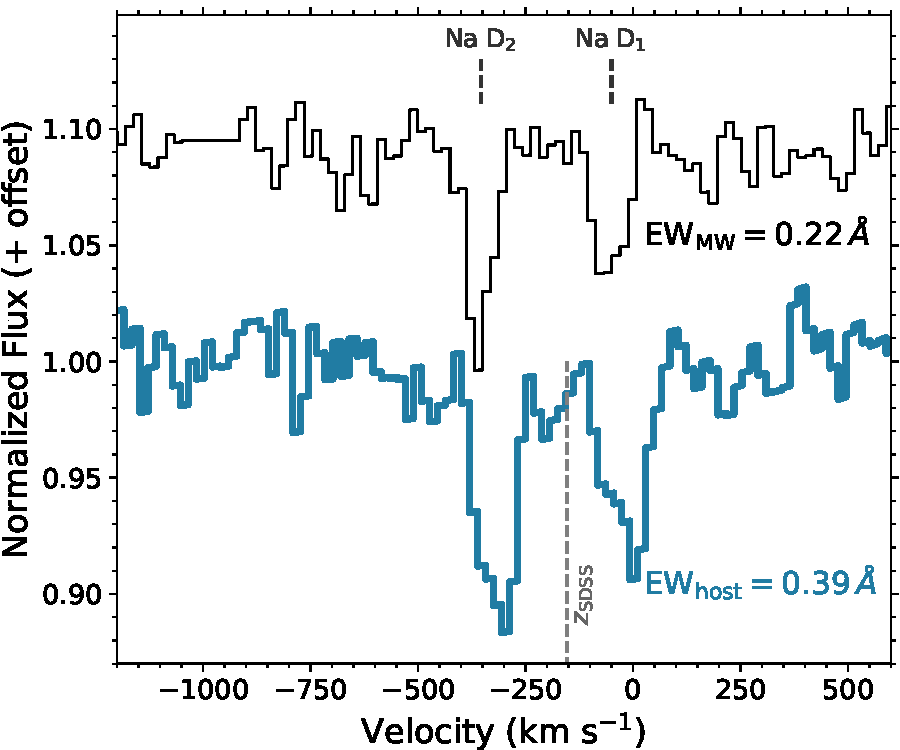
\includegraphics[width=3.5in]{./figures/NaD.pdf}
    %
    \caption{Zoom-in on our moderate resolution MMT+Binospec spectrum of \sn\
    highlighting absoprtion due to \ion{Na}{I} D in the host galaxy,
    NGC\,4441 (blue solid line), and the Milky Way (thin black line). The
    velocity scale is centered on the D$_2$ line in NGC\,4441, with the SDSS
    redshift shown via the vertical dashed line. No shift has been applied to
    the Milky Way lines. The \ion{Na}{I} D lines, which serve as a proxy for
    dust-obscuration along the line of sight (e.g.,
    \citep{Poznanski12,Phillips13}) are weak, indicating a relatively small
    amount of reddening. }
    %
    \label{fig:NaD}
\end{figure}

\subsection{Photometric Analysis}

We estimate the time of first light, \tfl, for \sn\ following the procedure
described in \citet{Miller20}. Briefly, \citet{Miller20} model the early
emission from a SN Ia as a power-law in time, $f \propto (t -
t_\mathrm{fl})^\alpha$, where $f$ is the flux, $t$ is time, and $\alpha$ is
the power-law index. \tfl\ is assumed to be the same everywhere in the
optical, allowing us to simultaneously fit observations in each of the ZTF
filters.

An important caveat for \sn\ is that the observed early decline in the light
curve clearly does not follow the simple power-law model, and thus these
observations must be masked when performing the fit. We conservatively
exclude observations from the first two nights of ZTF detection from the fit
(this choice is conservative as it is unclear when the mechanism that powers
the initial bump in \sn\ no longer significantly contributes to the flux in
the \gztf\ and \rztf\ filters). From the fit we find \tfl$ = -17.5
\pm^{1.0}{1.3}$\,d relative to \tbmax (we know \tfl$ < 17.4$\,d based on the
discovery detection in \citealt{Itagaki19} meaning a portion of the posterior
distribution for our model cannot be correct). We also find $\alpha_g = 2.15
\pm^{0.49}{0.36}$ and $\alpha_g = 1.91 \pm^{0.42}{0.31}$. These values are
typical of the normal SNe Ia studied in \citet{Miller20}. If we only exclude
the first observation from the model fit we find significantly different
results with a rise time that increases by $\sim$5\,d and power-law indicies
that increase by $\gtrsim$1.


\sn\ does not exhibit 


\begin{figure}
    \centering
    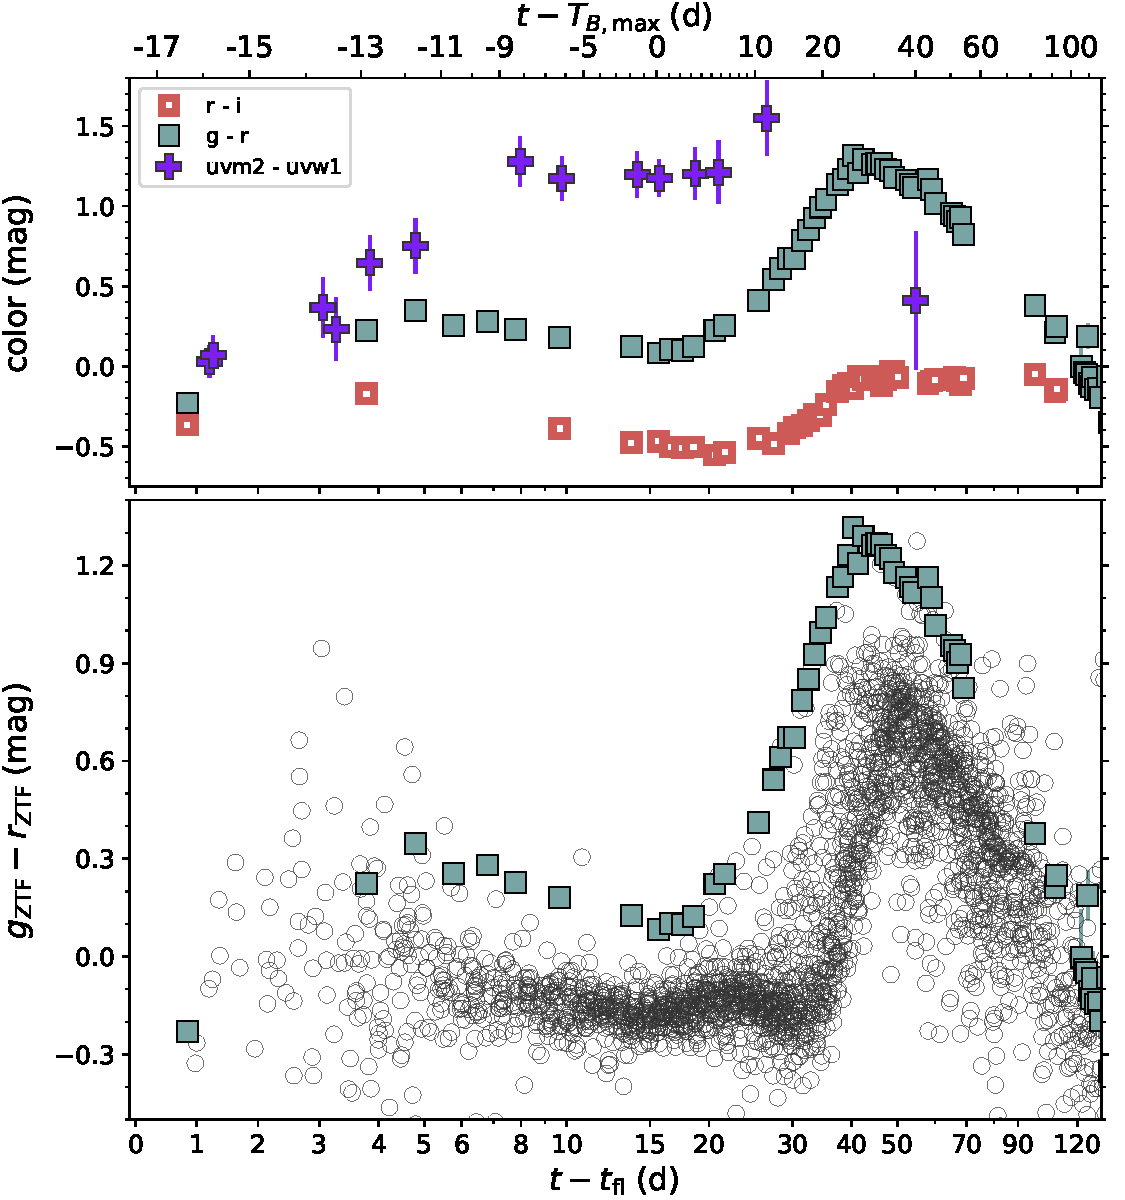
\includegraphics[width=3.5in]{./figures/P48_colors.pdf}
    %
    \caption{Color evolution of \sn.}
    %
    \label{fig:colors}
\end{figure}


\begin{figure}
    \centering
    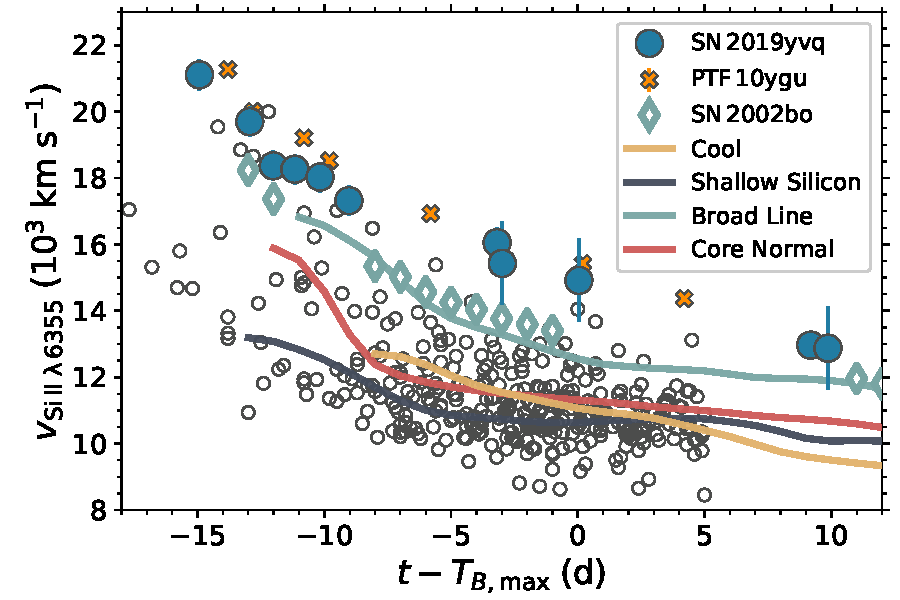
\includegraphics[width=3.5in]{./figures/vel_evolution.pdf}
    %
    \caption{Velocity evolution of \sn.}
    %
    \label{fig:vel_evo}
\end{figure}


\aam{\kate{$\longrightarrow$ spectral comparison}}

\begin{figure*}
    \centering
    \includegraphics[width=6.5in]{./figures/spec_comp.pdf}
    %
    \caption{Spectral comparison of \sn\ to other Cool and Broad Line SNe Ia.}
    %
    \label{fig:spec_comp}
\end{figure*}

\stockholm{Light curve fitting (SNOOPY, SALT2, etc?}

\aam{\stockholm{Host Galaxy}}



\section{Comparison to Models}\label{sec:models}

\abi{Best matching double det models}


\section{Rate of Thick He Shell Double Detonation Events}\label{sec:rates}

\textbf{This may not actually be a thick shell}

\aam{Use rough numbers from CLU and simple binomial calculation}

\section{Discussion and Conclusion}\label{sec:conclusions}

\todo{be clever}

\acknowledgements

This work is based on observations obtained with the Samuel Oschin Telescope
48-inch and the 60-inch Telescope at the Palomar Observatory as part of the
Zwicky Transient Facility project. ZTF is supported by the National Science
Foundation under Grant No. AST-1440341 and a collaboration including Caltech,
IPAC, the Weizmann Institute for Science, the Oskar Klein Center at Stockholm
University, the University of Maryland, the University of Washington,
Deutsches Elektronen-Synchrotron and Humboldt University, Los Alamos National
Laboratories, the TANGO Consortium of Taiwan, the University of Wisconsin at
Milwaukee, and Lawrence Berkeley National Laboratories. Operations are
conducted by COO, IPAC, and UW.

\software{
          \texttt{astropy} \citep{Astropy-Collaboration13},
          \texttt{scipy} \citep{Jones01}, 
          \texttt{matplotlib} \citep{Hunter07},
          \texttt{pandas} \citep{McKinney10},
        %   \texttt{emcee} \citep{Foreman-Mackey13},
        %   \texttt{corner} \citep{Foreman-Mackey16},
          \texttt{SALT2} \citep{Guy07},
          \texttt{sncosmo} \citep{Barbary16}
          }

%% For this sample we use BibTeX plus aasjournals.bst to generate the
%% the bibliography. The sample63.bib file was populated from ADS. To
%% get the citations to show in the compiled file do the following:
%%
%% pdflatex sample63.tex
%% bibtext sample63
%% pdflatex sample63.tex
%% pdflatex sample63.tex

\bibliography{/Users/adamamiller/Documents/tex_stuff/papers}
\bibliographystyle{aasjournal}

%% This command is needed to show the entire author+affiliation list when
%% the collaboration and author truncation commands are used.  It has to
%% go at the end of the manuscript.
%\allauthors

%% Include this line if you are using the \added, \replaced, \deleted
%% commands to see a summary list of all changes at the end of the article.
%\listofchanges

\begin{deluxetable*}{ccccc}
\tabletypesize{\scriptsize}
\tablewidth{0pt}
\tablecaption{Log of Spectroscopic Observations for SN~2019yvg.\label{tab:spectra}}
\tablehead{
\colhead{Date (UT)}&
\colhead{MJD}&
\colhead{Phase$^{*}$}&
\colhead{Telescope+Instrument}&
\colhead{Range}\\
\colhead{}&
\colhead{(days)}&
\colhead{(days)}&
\colhead{}&
\colhead{(\AA)}}
\startdata
31 Dec 2019 &  58848.273298   &    &  LT+SPRAT$^{*}$ &  4000--9000?   \\
03 Jan 2020 &     &     &  LT+SPRAT$^{*}$ &  4000--9000   \\
04 Jan 2020 &     &     &  LT+SPRAT &  4000--9000   \\
12 Jan 2020 &     &     &  LT+SPRAT &  4000--9000   \\
12 Jan 2020 &     &     &  LT+SPRAT  &  4000--9000   \\
15 Jan 2020 &     &     &  P60+SEDM$^{**}$ &  4000--9000   \\
18 Jan 2020 &     &     &  P60+SEDM &  4000--9000   \\
24 Jan 2020 &     &     &  MMT+Binospec$^{***}$ &  4000--9000   \\
25 Jan 2020 &     &     &  Keck+LRIS$^{****}$ &  4000--9000   \\
27 Jan 2020 &     &     &  P60+SEDM  &  4000--9000   \\
29 Jan 2020 &     &     &  NOT+ALFOSC$^{******}$ &  4000--9000   \\
01 Feb 2020 &     &     &  P60+SEDM &  4000--9000   \\
\enddata
\tablenotetext{*}{Liverpool Telescope}
%\tablenotetext{**}{}
%\tablenotetext{***}{}
\end{deluxetable*}



\end{document}